\chapter{Turingmaschinen}
\label{sec:turingmachine}
\index{Turingmaschine}
\index{Church-Turing-These}
\newcommand{\blank}{b}
%
Alan Turing (\life{1912}{1954}) machte sich viele Gedanken rund um mathematische Beweise und mechanische Prozesse. Er fragte sich, ob eine automatisierte Beweisführung von mathematischen Formeln möglich ist und konzipierte hierfür ein Maschinenkonzept. Die \emph{a-machine}~\cite{Turing01011937} (oder heutzutage als \emph{Turingmaschine} bezeichnet) wurde zum Referenzmodell der Theoretischen Informatik, welche auf einem praktikablen Weg zeigt, wo die Grenzen von Berechenbarkeit liegen und was automatisiert werden kann. Die Church-Turing-These behauptet, dass auch andere Konzepte wie das $\lambda$-Kalkül von Alonzo Church (welches zur selben Zeit entstanden ist) bezüglich Berechenbarkeit äquivalent sind:
%
\begin{quotation}
 Die Klasse der intuitiv berechenbaren Funktionen ist genau die Klasse der Turing-berechenbaren (dh. durch eine Turingmaschine berechenbare) Funktionen. \\
 ---Die Church-Turing-These
\end{quotation}
%
\section{Definition}
\index{Zustand (Turingmaschine)}
\index{Band (Turingmaschine)}
\index{Übergangsfunktion}
%
Eine Turingmaschine ist formal betrachtet ein 7-Tupel.
\begin{equation}
  \text{TM} = (Q, \Gamma, \blank, \Sigma, \delta, q_0, F)
\end{equation}
%
\begin{description}
 \item[$Q$] Eine endliche, nicht-leere Menge an Zuständen, die die Turingmaschine annehmen kann.
 \item[$\Gamma$] Eine endliche, nicht-leere Menge an Zeichen, die auf dem Band verwendet werden können.
 \item[$\blank$] Das Blanksymbol, welches den Initialzustand unbeschriebener Stellen beschreibt.
 \item[$\Sigma$] Eine endliche Menge an Zeichen, welche auf dem Band vorhanden sind.
 \item[$\delta$] Die Übergangsfunktion.
 \item[$q_0$] Ein Anfangszustand der TM.
 \item[$F$] Eine Menge von Endzuständen. Wird einer dieser Zustände erreicht, hält die Turingmaschine an.
\end{description}
%
Dabei gelten folgende Relationen zwischen den Elementen:
\begin{displaymath}
  \blank \in \Gamma \setminus \Sigma  \qquad
  \Sigma \subset \Gamma  \mathspace  \blank \in \Gamma  \qquad
\end{displaymath}
\begin{displaymath}
  q_0 \in Q \setminus F \qquad
  F \subset Q
\end{displaymath}

\section{Funktionsweise}
%
\begin{figure}[ht]
 \begin{center}
  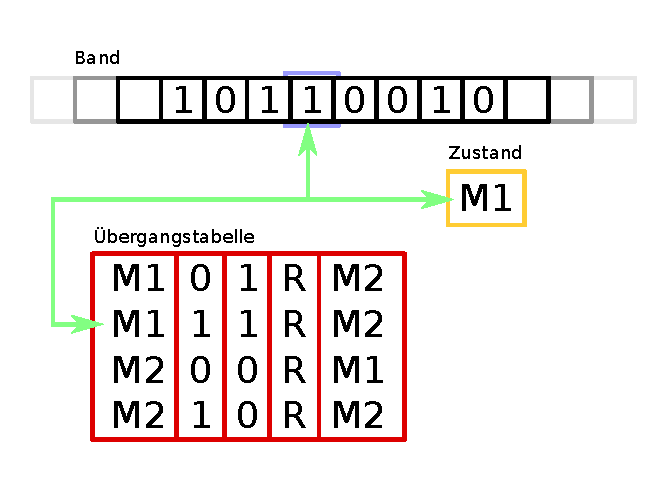
\includegraphics{img/turingmachine_visualization.pdf}
  \caption{Die Funktionsweise einer Turingmaschine visualisiert.}
  \label{fig:tm_vis}
 \end{center}
\end{figure}
%
In Abbildung~\ref{fig:tm_vis} ist der Aufbau einer Turingmaschine visualisiert. Die Turingmaschine besitzt ein unendlich langes \emph{Band} (schwarz) auf welchem Zeichen aus dem Alphabet $\Gamma$ stehen. Der \emph{Cursor} (blau) befindet sich an einer bestimmten Stelle auf diesem Band und liest und schreibt Zeichen. Basierend auf der Information in welchem \emph{Zustand} (orange) sich die Turingmaschine befindet und welches \emph{Zeichen gelesen} wurde, wird eine Zeile in der \emph{Übergangstabelle} (rot) ausgewählt, die dann den Zustandübergang definiert.

Die Turingmaschine besitzt eine initiale Konfiguration. Als Konfiguration bezeichnet man das Tupel (Zustand, Band, Cursor). Die abgebildeten Turingmaschine befindet sich in einem Zustand M1, auf dem Band befinden sich die Zeichen 10110010 (aus dem Alphabet $\Sigma$) und der Cursor ist links der Mitte positioniert. Dies sei unsere initiale Konfiguration. Die weiteren Konfigurationen lassen sich durch schrittweise Ausführung der Instruktionen ableiten. \\
Aufgrund der Konfiguration können wir jetzt in der Übergangstabelle nachschlagen, welche Instruktion ausgeführt werden soll. Eine Zeile der Spalte besteht dabei aus 5 Werten: Ausgangszustand, gelesenes Zeichen, geschriebenes Zeichen, Bewegung und nächster Zustand. Dies bedeutet in Zeile~2 stimmt die Konfiguration mit den Werten überein: Wir befinden uns im Zustand M1 (ja, in diesem befinden wir uns gerade) und lesen das Zeichen ,,1`` (ja, wurde vom Cursor gelesen). Dementsprechend ist eine ,,1`` an diese Position am Band zu schreiben, nach rechts (,,R``) zu fahren und in den Zustand ,,M2`` zu wechseln. Wenn wir den nachfolgenden Schritt beobachten, wird die Zeile 3 ausgeführt: Im Zustand ,,M2`` wurde das Zeichen ,,0`` gelesen, wird das Zeichen ,,0`` geschrieben, der Cursor nach rechts (,,R``) bewegt und in den Zustand ,,M1`` gewechselt.

Erreicht die Turingmaschine einen der definierten Endzustände, wird die Eingabe als ,,akzeptiert`` (Ja) interpretiert. Kommt die Turingmaschine in einen undefinierten Zustand, wird die Eingabe ,,abgelehnt`` (Nein).

Durch das Wechseln von Zuständen und das Speichern von Zeichen auf dem Band können Daten verarbeitet werden. Der Input und Output eines ablaufenden Algorithmus' bildet die Initial- und Endkonfiguration der Turingmaschine. Die Logik bzw. das Programm ist in der Übergangstabelle kodiert. Es ist im Allgemeinen nicht möglich aus der Problembeschreibung den entsprechenden Algorithmus zu generieren, der das Problem entscheidet. Dies begründet das Tätigkeitsfeld eines Programmierers und erfordert seine menschliche Kreativität.

Eine Turingmaschine, die eine Bewegung ,,Stop`` unterstützt ist gleich mächtig wie eine Turingmaschine, die es nicht unterstützt. Hierfür muss die Anzahl der Zustände (in denen ein Stop gebraucht wird) verdoppelt werden. In den folgenden Programmen verwenden wir die Bewegung ,,Stop``.

\section{Algorithmenbeispiele auf der Turingmaschine}
%
Im Folgenden werden 3 Algorithmen für 3 verschiedene Probleme vorgestellt, die wir auf einer Turingmaschine entscheiden werden. Sie folgen jeweils unterschiedlichen Ideen und sollen dem Leser mögliche Lösungsansätze für andere äquivalente Probleme illustrieren.

\subsection{Algorithmus: Gerade oder ungerade Anzahl}
\index{Gerade oder ungerade Anzahl (Algorithmus)}
%
Gegeben sei eine Turingmaschine. Auf dem Band befindet sich eine beliebige Sequenz von Nullen (0) und Einsen (1). Der Cursor befindet sich auf der linkesten Ziffer. Gehe in den Endzustand ,,Even`` wenn sich eine gerade Anzahl an Ziffern auf dem Band befinden. Gehe in den Endzustand ,,Odd`` wenn sich eine ungerade Anzahl an Ziffern auf dem Band befinden. Die Position des Cursors in den Endzuständen ist nicht spezifiziert. Das Band muss im Endzustand gleich wie am Anfang aussehen. Schreibe das Programm der Turingmaschine, um dieses Problem zu entscheiden.

\textbf{Lösung (Tabelle~\ref{tab:odd_even}).} Der Lösungsansatz beruht darauf zwischen den zwei Zuständen ,,Even`` und ,,Odd`` zu alternieren, wobei der entsprechende Zustand repräsentiert, ob eine gerade oder ungerade Anzahl von Zeichen bisher gelesen wurde. Zu beachten ist weiters, dass die Sequenz auch die Länge $0$ umfasst und daher der Fall abgedeckt werden muss, falls sich kein Zeichen (bzw. das Blanksymbol) unter dem Startzustand befindet.
%
\begin{table}
 \begin{center}
  \begin{tabular}{ccccc}
   \hline
    Zustand & Lesen     & Schreiben & Bewegung & neuer Zustand \\
   \hline \hline
    Start   & $\square$ & $\square$ & Stop     & Even \\
    Start   & 0         & 0         & Rechts   & Odd \\
    Start   & 1         & 1         & Rechts   & Odd \\
    Even    & $\square$ & $\square$ & Stop     & Even \\
    Even    & 0         & 0         & Rechts   & Odd \\
    Even    & 1         & 1         & Rechts   & Odd \\
    Odd     & $\square$ & $\square$ & Stop     & Odd \\
    Odd     & 0         & 0         & Rechts   & Even \\
    Odd     & 1         & 1         & Rechts   & Even \\
   \hline
  \end{tabular}
  \caption{Eine Übergangstabelle für ,,Gerade oder ungerade Anzahl``.}
  \label{tab:odd_even}
 \end{center}
\end{table}

\subsection{Algorithmus: 1en zählen}
\index{Einsen zählen (Algorithmus)}
%
Gegeben sei eine Turingmaschine. Auf dem Band befindet sich eine beliebige Sequenz von Nullen und Einsen (der Mindestlänge 1). Der Cursor befindet sich auf der linkesten Ziffer. Gesucht ist ein Algorithmus, welcher das Band mit Blanksymbolen überschreibt und genau so viele Einsen nebeneinander angeordnet schreiben soll, wie im String anfangs enthalten waren. Als Beispiel soll der Eingabestring ,,00101101`` zur Ausgabe ,,1111`` führen. Als weiteres Beispiel soll ,,10`` zu ,,1`` führen. Im Endzustand ,,End`` soll der Cursor auf der rechtesten 1 stehen.

\textbf{Lösung (Tabelle~\ref{tab:count_ones}).} Der Algorithmus folgt diesem Ablauf:
\begin{enumerate}
  \item Markiere Anfang (\^{}) und Ende (\$) mit zwei Hilfssymbolen
        (diese Markung wird in den Zuständen Start und Mark vorgenommen).
  \item Im Zustand \textit{Find} gehe nach rechts und suche die nächste 1.
        Ersetze sie mit einer 0 und gehe in Zustand \textit{Found} oder falls du keine 1 findest,
        finalisiere das Band.
  \item In den Zuständen \textit{Found}, \textit{Write} und \textit{Return} wird das Symbol
        auf der rechten Seite des Hilfssymbols \$ hinzugefügt und es wird zurück zur linken Seite gegangen.
  \item Beim Finalisieren lösche die Hilfssymbole \^{} und \$ und die Anfangssequenz von Nullen und Einsen
        vom Band. Gehe an die rechteste Position des Ergebnisses.
\end{enumerate}
%
\begin{table}
 \begin{center}
  \begin{tabular}{ccccc}
   \hline
    Zustand & Lesen     & Schreiben & Bewegung & neuer Zustand \\
   \hline \hline
    Start   & $\square$ & \$        & Links    & Mark \\
    Start   & 0         & 0         & Rechts   & Start \\
    Start   & 1         & 1         & Rechts   & Start \\
    Mark    & $\square$ & \^{}      & Rechts   & Find \\
    Mark    & 0         & 0         & Links    & Mark \\
    Mark    & 1         & 1         & Links    & Mark \\
    Find    & 0         & 0         & Rechts   & Find \\
    Find    & 1         & 0         & Rechts   & Found \\
    Find    & \$        & \$        & Links    & Finalize \\
    Found   & 0         & 0         & Rechts   & Found \\
    Found   & 1         & 1         & Rechts   & Found \\
    Found   & \$        & \$        & Rechts   & Write \\
    Write   & $\square$ & 1         & Links    & Return \\
    Write   & 1         & 1         & Rechts   & Write \\
    Return  & 0         & 0         & Links    & Return \\
    Return  & 1         & 1         & Links    & Return \\
    Return  & \$        & \$        & Links    & Return \\
    Return  & \^{}      & \^{}      & Rechts   & Find \\
    Finalize& 0         & 0         & Links    & Finalize \\
    Finalize& 1         & 1         & Links    & Finalize \\
    Finalize& \^{}      & $\square$ & Rechts   & Delete \\
    Delete  & 0         & $\square$ & Rechts   & Delete \\
    Delete  & 1         & $\square$ & Rechts   & Delete \\
    Delete  & \$        & $\square$ & Rechts   & Result \\
    Result  & $\square$ & $\square$ & Stop     & End \\
    Result  & 1         & 1         & Rechts   & Result \\
   \hline
  \end{tabular}
  \caption{Eine Zustandstabelle für ,,Einsen zählen``.}
  \label{tab:count_ones}
 \end{center}
\end{table}

\subsection{Algorithmus: Minimum von 3 2-bit Zahlen}
\index{Minimum von 2-bit Zahlen (Algorithmus)}
%
Gegeben sei eine Turingmaschine. Auf dem Band befinden sich 6 Nullen oder Einsen. Diese sind als 3 2-bit Zahlen zu interpretieren. Schreibe rechts von diesen Zahlen jenen Wert, der das Minimum der 3 Zahlen repräsentiert und lasse das restliche Band im Anfangszustand. Der Startzustand sei ,,Start`` und der Endzustand sei ,,End``. Die initiale Cursorposition sei die linkeste Ziffer. Im Endzustand soll der Cursor ganz rechts sein.

\textbf{Lösung (Tabelle~\ref{tab:min_3bit}).} Unser Lösungsansatz beruht auf der Idee, dass wir sämtliche relevanten Informationen des Inputs in den Zuständen speichern. Wir modifizieren das Band nicht (d.h. gelesene und geschriebene Zeichen sind stets ident außer wir schreiben das Ergebnis) und die Bewegung geht stets nach rechts (außer wir terminieren). Wir lesen Ziffer für Ziffer ein und wechseln in einen entsprechenden Zustand. So wird etwa in dem Startzustand bei einem gelesenen $1$ in den Zustand $001$ gewechselt, um uns zu merken dass das kleinste Minimum $00$ war (wir haben bisher noch keine Zahl gelesen und daher wird die niedrigste Zahl $00$ verwendet) und mit der zusätzlichen $1$ merken wir uns das letzte gelesene Symbol. Dies ist bei allen Zuständen, die aus 3 Ziffern bestehen gleichartig. Wir müssen dabei in jenen Zustand wechseln, welcher das Maximum der zwei Zustände repräsentiert, die wir durch den aktuellen Zustand und das gelesene Zeichen kodiert haben. Haben wir eine gerade Anzahl an Zeichen gelesen, befinden wir uns in einem Zustand aus 2 Ziffern und sonst in einem Zustand aus 3 Ziffern. Kommen wir auf ein Blanksymbol, schreiben wir jene Zahl, die wir als Minimum im Namen des Zustands gespeichert haben.
%
\begin{table}
 \begin{center}
  \begin{tabular}{ccccc}
   \hline
    Zustand & Lesen     & Schreiben & Bewegung & neuer Zustand \\
   \hline \hline
    Start   & 0         & 0         & Rechts   & 000 \\
    Start   & 1         & 1         & Rechts   & 001 \\
    000     & 0         & 0         & Rechts   & 00 \\
    000     & 1         & 1         & Rechts   & 01 \\
    001     & 0         & 0         & Rechts   & 10 \\
    001     & 1         & 1         & Rechts   & 11 \\
    010     & 0         & 0         & Rechts   & 01 \\
    010     & 1         & 1         & Rechts   & 01 \\
    011     & 0         & 0         & Rechts   & 10 \\
    011     & 1         & 1         & Rechts   & 11 \\
    100     & 0         & 0         & Rechts   & 10 \\
    100     & 1         & 1         & Rechts   & 10 \\
    101     & 0         & 0         & Rechts   & 10 \\
    101     & 1         & 1         & Rechts   & 11 \\
    110     & 0         & 0         & Rechts   & 11 \\
    110     & 1         & 1         & Rechts   & 11 \\
    111     & 0         & 0         & Rechts   & 11 \\
    111     & 1         & 1         & Rechts   & 11 \\
    00      & $\square$ & 0         & Rechts   & 0 \\
    00      & 0         & 0         & Rechts   & 000 \\
    00      & 1         & 0         & Rechts   & 001 \\
    01      & $\square$ & 0         & Rechts   & 0 \\
    01      & 0         & 0         & Rechts   & 010 \\
    01      & 1         & 1         & Rechts   & 011 \\
    10      & $\square$ & 1         & Rechts   & 0 \\
    10      & 0         & 0         & Rechts   & 100 \\
    10      & 1         & 1         & Rechts   & 101 \\
    11      & $\square$ & 1         & Rechts   & 1 \\
    11      & 0         & 0         & Rechts   & 110 \\
    11      & 1         & 1         & Rechts   & 111 \\
    0       & $\square$ & 0         & Stop     & End \\
    1       & $\square$ & 1         & Stop     & End \\
   \hline
  \end{tabular}
  \caption{Eine Zustandstabelle für ,,Minimum von 3 2-bit Zahlen``.}
  \label{tab:min_3bit}
 \end{center}
\end{table}

\section{Theoretische Erkenntnisse}
\subsection{Universelle Turingmaschine}
\index{Universelle Turingmaschine}
%
Unter einer \emph{universellen Turingmaschine} versteht man eine Turingmaschine, welche als Parameter\footnote{Unter Parameter im Kontext einer Turingmaschine versteht man einen Wert, welcher bereits auf das Band kodiert wurde, bevor die Turingmaschine gestartet wurde.} eine andere Turingmaschine entgegen nimmt und nachfolgend die einzelnen Schritte der Turingmaschine berechnet. Dabei befinden sich alle Informationen wie der aktuelle Zustand, das Band und das Programm auf dem Band der universellen Turingmaschine. Wird ein Befehl der simulierten Turingmaschine ausgeführt, wird am Band nach der entsprechenden Instruktion nachgeschlagen und der Befehl ausgeführt.

Die genaue Implementierung wird hier nicht weiter präzisiert, da es sich nur um Überlegungen hinsichtlich Kodierungen handelt.
%
\subsection{Mehrbandturingmaschinen}
\index{Mehrbandturingmaschine}
%
Eine Erweiterung der Turingmaschine besteht darin mehr als 1 Band zu verwenden. Dies hilft insbesondere bei der Organisation der Daten bei der Implementierung von Algorithmen. Betrachten wir etwa ein Graphenproblem, hilft es beispielweise auf einem Band den aktuell betrachteten Knoten zu speichern und auf den weiteren Bändern zwei anliegende Kanten. In dem Fall müssen wir die Wanderungen nicht ausformulieren, wenn wir die Bänderdaten von einem anderen Band lesen wollen und diese Bänder nebeneinander angeordnet werden.

Jede Mehrbandturingmaschine kann durch eine Turingmaschine mit 1 Band simuliert werden.

Die Frage, die sich jedoch stellt, ist: Hat diese Erweiterung Auswirkungen auf die Komplexität der Probleme? Wie es sich herausstellt, handelt es sich nur um einen polynomiallen Mehraufwand.
%
\subsection{Nicht-Determinismus}
\label{sec:nondeterminism}
\index{Nicht-Determinismus}
\index{Orakel (Turingmaschine)}
%
Der Nichtdeterminismus ist ein wichtiges Konzept für die theoretische Informatik. Grundsätzlich handelt es sich bei der Übergangsfunktion der Turingmaschine um eine Abbildung des gelesenen Zeichens und des aktuellen Zustands auf den neuen Zustand, das zu schreibende Zeichen und eine Bewegung. Nichtdeterminismus beschreibt den Zustand eines Systems in dem der Übergang von einem Zustand der Maschine in den nächsten Zustand nicht wohldefiniert und eindeutig ist. In anderen Worten auch: Für eine gegebene Konfiguration der Turingmaschine gibt es mehrere Möglichkeiten in den nächsten Zustand zu kommen.

Im Kontext der Komplexitätstheorie spricht man bei Nichtdeterminismus von den sogenannten \emph{Orakelturingmaschinen}. Liegen mehrere Zustandübergänge für eine Konfiguration vor, befragt die Turingmaschine die (zur Verfügung stehende) Orakelturingmaschine. Diese antwortet stets mit jenem Übergang, welcher direkt zur richtigen Lösung führt. Diese Hervorsagefähigkeit begründet ihren Namen ,,Orakel``.
%
\subsection{Halteproblem}
\index{Halteproblem}
%
\index{Turing-berechenbar}
Wichtig ist es zu verstehen, dass es eine Menge an Funktionen\footnote{Wir verwenden hier den Begriff ,,Funktion`` wie den Begriff ,,Algorithmus``. Was in diesem Dokument stets ein Algorithmus ist, bezeichnete Alan Turing als Funktion.} gibt, die mit einer Turingmaschine berechenbar sind und welche, die nicht \emph{Turing-berechenbar} sind. Die Menge aller Funktionen teilt sich also in jene der Turing-berechenbaren und nicht-Turing-berechenbaren. Wir haben jetzt Turing-berechenbare Probleme kennen gelernt\footnote{Erkennbar daran, dass wir ein Problem analysiert, eine entsprechende Implementierung formuliert und dann einen Algorithmus entwickelt haben, der uns das Problem entscheidet.}. Welche nicht-Turing-berechenbare Funktionen gibt es? Der bekannteste Vertreter dieser ist das Halteproblem.

Das Halteproblem stellt uns die Frage, ob wir mit einer universellen Turingmaschine $U$ entscheiden können, ob eine andere Turingmaschine $M$ beim Ausführen eines beliebigen Algorithmus terminieren wird. Dieses Problem kann für einen allgemeinen Algorithmus nicht entschieden werden und ist daher nicht Turing-berechenbar.
